\documentclass[]{article}
\usepackage{lmodern}
\usepackage{amssymb,amsmath}
\usepackage{ifxetex,ifluatex}
\usepackage{fixltx2e} % provides \textsubscript
\ifnum 0\ifxetex 1\fi\ifluatex 1\fi=0 % if pdftex
  \usepackage[T1]{fontenc}
  \usepackage[utf8]{inputenc}
\else % if luatex or xelatex
  \ifxetex
    \usepackage{mathspec}
    \usepackage{xltxtra,xunicode}
  \else
    \usepackage{fontspec}
  \fi
  \defaultfontfeatures{Mapping=tex-text,Scale=MatchLowercase}
  \newcommand{\euro}{€}
\fi
% use upquote if available, for straight quotes in verbatim environments
\IfFileExists{upquote.sty}{\usepackage{upquote}}{}
% use microtype if available
\IfFileExists{microtype.sty}{%
\usepackage{microtype}
\UseMicrotypeSet[protrusion]{basicmath} % disable protrusion for tt fonts
}{}
\ifxetex
  \usepackage[setpagesize=false, % page size defined by xetex
              unicode=false, % unicode breaks when used with xetex
              xetex]{hyperref}
\else
  \usepackage[unicode=true]{hyperref}
\fi
\hypersetup{breaklinks=true,
            bookmarks=true,
            pdfauthor={},
            pdftitle={},
            colorlinks=true,
            citecolor=blue,
            urlcolor=blue,
            linkcolor=magenta,
            pdfborder={0 0 0}}
\urlstyle{same}  % don't use monospace font for urls
\usepackage{graphicx,grffile}
\makeatletter
\def\maxwidth{\ifdim\Gin@nat@width>\linewidth\linewidth\else\Gin@nat@width\fi}
\def\maxheight{\ifdim\Gin@nat@height>\textheight\textheight\else\Gin@nat@height\fi}
\makeatother
% Scale images if necessary, so that they will not overflow the page
% margins by default, and it is still possible to overwrite the defaults
% using explicit options in \includegraphics[width, height, ...]{}
\setkeys{Gin}{width=\maxwidth,height=\maxheight,keepaspectratio}
\setlength{\parindent}{0pt}
\setlength{\parskip}{6pt plus 2pt minus 1pt}
\setlength{\emergencystretch}{3em}  % prevent overfull lines
\providecommand{\tightlist}{%
  \setlength{\itemsep}{0pt}\setlength{\parskip}{0pt}}
\setcounter{secnumdepth}{0}

\date{}

% Redefines (sub)paragraphs to behave more like sections
\ifx\paragraph\undefined\else
\let\oldparagraph\paragraph
\renewcommand{\paragraph}[1]{\oldparagraph{#1}\mbox{}}
\fi
\ifx\subparagraph\undefined\else
\let\oldsubparagraph\subparagraph
\renewcommand{\subparagraph}[1]{\oldsubparagraph{#1}\mbox{}}
\fi
\title {Marker based localization \\ [10pt]
	Shape Detection  \\[25pt] Team members }
\author {Niharika Jayanthi \and Dheeraj Kamath}
\begin{document}
\maketitle
\begin{center}
	\begin{large}
		Under the guidance of\\
		\textbf{Sanam Shakya}\\
		\vspace{0.5in}
	\end{large}
\end{center}
\section{Goal}\label{goal}

\emph{\textbf{In this chapter we will see,}} \\
* how to find various
properties of contours\\
* how to apply these properties\\
* we will learn
about : \textbf{cv2.contourArea()}, \textbf{cv2.arcLength()},
\textbf{cv2.approxPolyDP()}

\section{Theory}\label{theory}

Contours have various features like area, perimeter, moments etc which
can be used for various applications.

\subsection{Working principle}\label{working-principle}

1.\textbf{Contour Area} - The area of the object is found with the help
of moments. Area is calculated by zero order moment. For more details on
moments refer:
\href{https://github.com/eyantrainternship/eYSIP_2015_Marker_based_Robot_Localisation/wiki/Moments}{Moments}

\texttt{cv2.contourArea(contour,\ oriented)}

Parameters:\\
* \textbf{contour} -- Input vector of 2D points (contour vertices)\\
* \textbf{oriented} -- Oriented area flag. If it is true, the function
returns a signed area value, depending on the contour orientation
(clockwise or counter-clockwise). Using this feature you can determine
orientation of a contour by taking the sign of an area. By default, the
parameter is false, which means that the absolute value is returned.

2.\textbf{Contour Perimeter} - Used to find the arc length of the
contour.\\
\texttt{cv2.arcLength(curve,\ closed)}

Parameters:\\
* \textbf{curve} - Input vector of 2D points\\
* \textbf{closed} - Flag indicating whether the curve is closed or not

3.\textbf{ApproxPolyDP()} - This is used to obtain the number of points
found in the figure. \texttt{epsilon} is an accuracy parameter. A wise
selection of epsilon is needed to get the correct output.

\begin{verbatim}
 epsilon = 0.1*cv2.arcLength(cnt,True)
 approx = cv2.approxPolyDP(curve, epsilon, closed, approxCurve) 
\end{verbatim}

Parameters:\\
* \textbf{curve} -- Input vector of a 2D point.\\
* \textbf{approxCurve} -- Result of the approximation. The type should
match the type of the input curve. In case of C interface the
approximated curve is stored in the memory storage and pointer to it is
returned. epsilon -- Parameter specifying the approximation accuracy.
This is the maximum distance between the original curve and its
approximation.\\
* \textbf{closed} -- If true, the approximated curve is closed (its
first and last vertices are connected). Otherwise, it is not closed.

\section{Shape Detection}\label{shape-detection}

Using all these properties we will see how to detect shapes and display
the name of the shape at its center. All the shapes can be first
identified by the number of vertices and then for shapes with the shapes
with the same number of vertices we can use Hu moments based
matchShapes() function. We will be trying to detect the following
shapes:\\
\texttt{Triangle,\ Square,\ Rectangle,\ Parallelogram,\ Pentagon,\ Hexagon,\ Star\ and\ Circle.}\\
Since there are three shapes having four points we will compare the
return value of each of the shapes with the square. The output of
\texttt{cv2.matchShapes()} is a return value indicating the amount of
deviation from sample image. If ret = 0 its a square, if 0 \textless{}
ret \textless{} 0.5 its a rectangle and if ret \textgreater{} 0.5 its a
parallelogram. These values were obtained by trial and error basis.

\section{Code}\label{code}

\begin{verbatim}
#Importing modules
import cv2 
import numpy
import matplotlib.pyplot as plt

#Sample image for shapes with 4 vertices
img = cv2.imread('square.png')

#Reading the image from the user
inp_img = cv2.imread(raw_input("Enter the name of the unknown image:"))

#Converting to grayscale
gray = cv2.cvtColor(img, cv2.COLOR_BGR2GRAY)
gray1 = cv2.cvtColor(inp_img, cv2.COLOR_BGR2GRAY)

'''
OpenCV represents RGB images as multi-dimensional NumPy arrays…but in reverse
order!This means that images are actually represented in BGR order rather than
RGB!
'''
#Convert to RGB
inp_img = cv2.cvtColor(inp_img, cv2.COLOR_BGR2RGB)
img = cv2.cvtColor(img, cv2.COLOR_BGR2RGB)


#Thresholding
ret, thresh = cv2.threshold(gray, 0,255,0)
ret, thresh1 = cv2.threshold(gray1, 0,255,0)

#Using Canny for perfect edge detection
canny = cv2.Canny(img,100,200)

#Finding contours
contours,heirarchy = cv2.findContours(thresh, cv2.RETR_TREE, cv2.CHAIN_APPROX_SIMPLE)
cnt1 = contours[0]
contours1,heirarchy = cv2.findContours(thresh1, cv2.RETR_TREE, cv2.CHAIN_APPROX_SIMPLE)
cnt2 = contours1[0]


#Finding the centroid
for s in contours1:
    M = cv2.moments(s)
    cx = int(M['m10']/M['m00'])
    cy = int(M['m01']/M['m00'])


#####################Detection of shape#################################### 
font = cv2.FONT_HERSHEY_SIMPLEX

#Creating lists
a = []
b = []

#Finding vertices in input image
for i in contours1:
    approx = cv2.approxPolyDP(i,0.01*cv2.arcLength(i,True),True)
    print len(approx)
    x = len(approx)
    a.append(x)
print a    

#Finding vertices in sample image
for i in contours:
    approx = cv2.approxPolyDP(i,0.01*cv2.arcLength(i,True),True)
    print len(approx)
    x = len(approx)
    b.append(x)
print b      

 #Detection and display of name of shape
 for i in contours1:
    for m in a:
        for n in b:
             if m == 4 & n ==4:
                 ret = cv2.matchShapes(cnt1,cnt2,1,0.0)
                 print ret
            
                 if ret> 0.5:
                    print "Parallelogram"
                    cv2.drawContours(img,[i],0,(0,255,0),2)
                    cv2.putText(img,"Slight match",(50,50),font,1,(0,255,0),2)
                    cv2.putText(inp_img,"Parallelogram",(cx-20,cy),font,0.5,(0,0,255),2)
                    cv2.imshow('Compare',img)
                elif 0.3< ret < 0.5:
                    print "Rectangle"
                    cv2.drawContours(img,[i],0,(0,255,0),2)
                    cv2.putText(img,"Slight Match",(50,50),font,0.5,(0,0,255),2)
                    cv2.putText(inp_img,"Rectangle",(cx-20,cy),font,0.5,(0,0,255),2)
                    cv2.imshow('Compare',img)
                elif 0 < ret < 0.3:
                    print "Rhombus"
                    cv2.drawContours(img,[i],0,(0,255,0),2)
                    cv2.putText(img,"Slight Match",(50,50),font,0.5,(0,0,255),2)
                    cv2.putText(inp_img,"Rhombus",(cx-20,cy),font,0.5,(0,0,255),2)
                    cv2.imshow('Compare',img)
                else:
                    print "Square"
                    cv2.drawContours(img,[i],0,(0,255,0),2)
                    cv2.putText(img,"Perfect Match",(50,50),font,2,(0,0,255),2)
                    cv2.putText(inp_img,"Square",(cx-25,cy),font,1,(0,0,255),2)
                    cv2.imshow('Compare',img)
                
                
        
        
             elif m ==3:
                cv2.drawContours(inp_img,[i],0,(0,255,0),2)
                print "Input image is a triangle"
                cv2.putText(inp_img,"Triangle",(cx-20,cy),font,0.5,(0,0,255),2)
        
                        
            elif m ==5:
                print "pentagon"
                cv2.drawContours(inp_img,[i],0,(0,255,0),2)
                cv2.putText(inp_img,"Pentagon",(cx-20,cy),font,0.5,(0,0,255),2)
            
            elif m == 6:
                print "hexagon"
                cv2.drawContours(inp_img,[i],0,(0,255,0),2)
                cv2.putText(inp_img,"Hexagon",(cx-20,cy),font,0.5,(0,0,255),2)
        
        
            elif m == 7:
                print "Arrow"
                cv2.drawContours(inp_img,[i],0,(0,255,0),2)
                cv2.putText(img,"Arrow",(cx-20,cy),font,0.5,(0,0,255),2)
        
            elif m > 7:
                print "Circle"
                cv2.drawContours(inp_img,[i],0,(0,255,0),2)
                cv2.putText(inp_img,"Circle",(cx-20,cy),font,0.5,(0,255,0),2)
       

 #Plotting the image
 plt.subplot(121),plt.imshow(img), plt.title('Original image'),plt.set_cmap('bone')
 plt.xticks([]), plt.yticks([])
 plt.subplot(122),plt.imshow(inp_img),plt.title('Shape found'),plt.set_cmap('bone')
 plt.xticks([]), plt.yticks([])
 plt.show()
 cv2.waitKey(0)
 cv2.destroyAllWindows()
\end{verbatim}

If we input ``parallelogram.png'' we get:\\
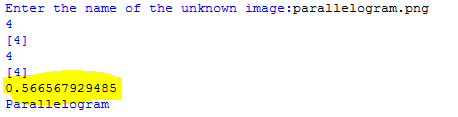
\includegraphics{ret.PNG}\\
The highlighted portion represents the return value.

\newpage
We get the following as output:\\
\begin{figure}[h]
	\centering
	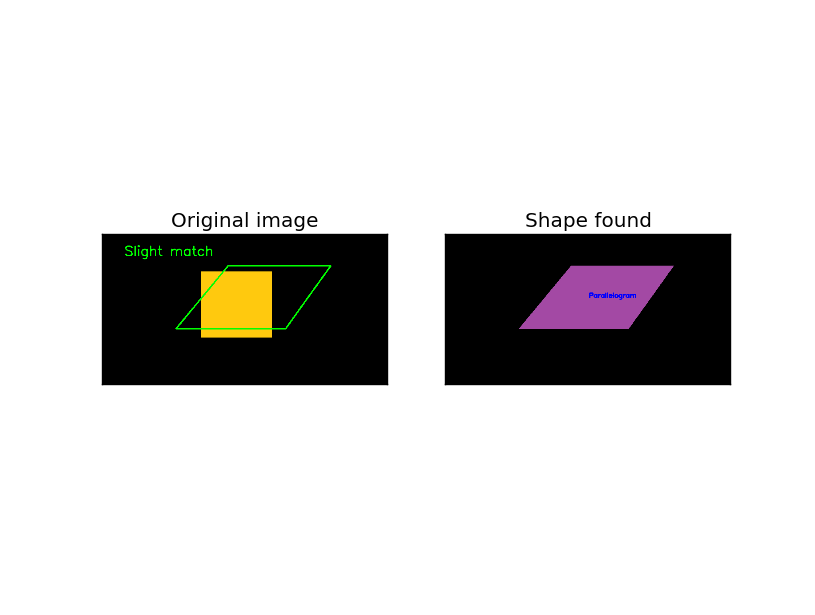
\includegraphics[width = 18cm]{shapes3.png}
	\caption{Shape detection}
\end{figure}

\section{Resources}\label{resources}

1. \href{http://opencv-python-tutroals.readthedocs.org/en/latest/py \\
\_tutorials/py\_imgproc/py\_contours/py\_contour\_features/py\\
\_contour\_features.html\#contour-features}{Contour features}\\
2. \href{http://docs.opencv.org/modules/imgproc/doc/structural\_analysis \\
\_and\_shape\_descriptors.html?highlight=findcontours\#arclength}{Contour Properties}

\end{document}
